\documentclass[]{report}   % List options between brackets

% List packages between braces
\usepackage[margin=1.2in]{geometry}
\usepackage{caption}              % Allows use of \caption* to omit ``Figure''
\usepackage{color}
\usepackage{enumerate}
\usepackage{float}                % Used for H placement permission to put figures in sections properly
\usepackage{graphicx}             % For rendering .eps images in document
\usepackage{listings}             % Used for syntax highlighting when including source code examples
\usepackage{titlesec}             % http://ctan.org/pkg/titlesec 
\usepackage{tikz}

% For changing the table of content entries in to hyperlinks
\usepackage[linktoc=all]{hyperref}
\hypersetup{colorlinks=true, linkcolor=blue}

% Type user-defined commands here
\renewcommand{\thesection}{}% Remove section references...
\renewcommand{\thesubsection}{\arabic{subsection}}%... from subsections

% Define custom colors
\definecolor{mygreen}{rgb}{0,0.6,0}
\definecolor{mygray}{rgb}{0.5,0.5,0.5}
\definecolor{mymauve}{rgb}{0.58,0,0.82}

% Set source code inclusion formatting
\lstset{%
  backgroundcolor=\color{white},   % choose the background color; you must add \usepackage{color} or \usepackage{xcolor}
  basicstyle=\footnotesize,        % the size of the fonts that are used for the code
  breakatwhitespace=false,         % sets if automatic breaks should only happen at whitespace
  breaklines=true,                 % sets automatic line breaking
  captionpos=b,                    % sets the caption-position to bottom
  commentstyle=\color{mygreen},    % comment style
  deletekeywords={\ldots},            % if you want to delete keywords from the given language
      %escapeinside={\%*}{*)},          % if you want to add LaTeX within your code
  extendedchars=true,              % lets you use non-ASCII characters; for 8-bits encodings only, does not work with UTF-8
  frame=single,                    % adds a frame around the code
  keepspaces=true,                 % keeps spaces in text, useful for keeping indentation of code (possibly needs columns=flexible)
  keywordstyle=\color{blue},       % keyword style
  language=Verilog,                 % the language of the code
  morekeywords={*,\ldots},            % if you want to add more keywords to the set
  numbers=left,                    % where to put the line-numbers; possible values are (none, left, right)
  numbersep=5pt,                   % how far the line-numbers are from the code
  numberstyle=\tiny\color{mygray}, % the style that is used for the line-numbers
  rulecolor=\color{black},         % if not set, the frame-color may be changed on line-breaks within not-black text (e.g. comments (green here))
  showspaces=false,                % show spaces everywhere adding particular underscores; it overrides 'showstringspaces'
  showstringspaces=false,          % underline spaces within strings only
  showtabs=false,                  % show tabs within strings adding particular underscores
  stepnumber=1,                    % the step between two line-numbers. If it's 1, each line will be numbered
  stringstyle=\color{mymauve},     % string literal style
  tabsize=2,                       % sets default tabsize to 2 spaces
title=\lstname}                   % show the filename of files included with \lstinputlisting; also try caption instead of title

\begin{document}
\raggedright{}  % Don't allow text to be spread to the right margin

\title{Tournament Predictor}   % type title between braces
\author{Andrei Kniazev\\
  Benjamin Hunstman\\
  Michael Walton\\
  Kevin Bedrossian\\
}         % type author(s) between braces
\date{March 14, 2014}    % type date between braces
\maketitle

\begin{abstract}
  A branch predictor modeled using the Alpha 21264 microprocessor tournament predictor is simulated in software in order to demonstrate the performance of this particular technique of branch prediction.
  The predictor simply makes both a local prediction and a global prediction, and uses a choice prediction that predicts which of the two prediction techniques will be correct.
\end{abstract}

\tableofcontents

\chapter{Design}
A branch predictor modeled using the Alpha 21264 microprocessor tournament predictor is simulated in software in order to demonstrate the performance of this particular technique of branch prediction.
The predictor simply makes both a local prediction and a global prediction, and uses a choice prediction that predicts which of the two prediction techniques will be correct.
Once the branch is taken or not taken we update the prediction tables as well as the path history.

\begin{figure}
\begin{center}
  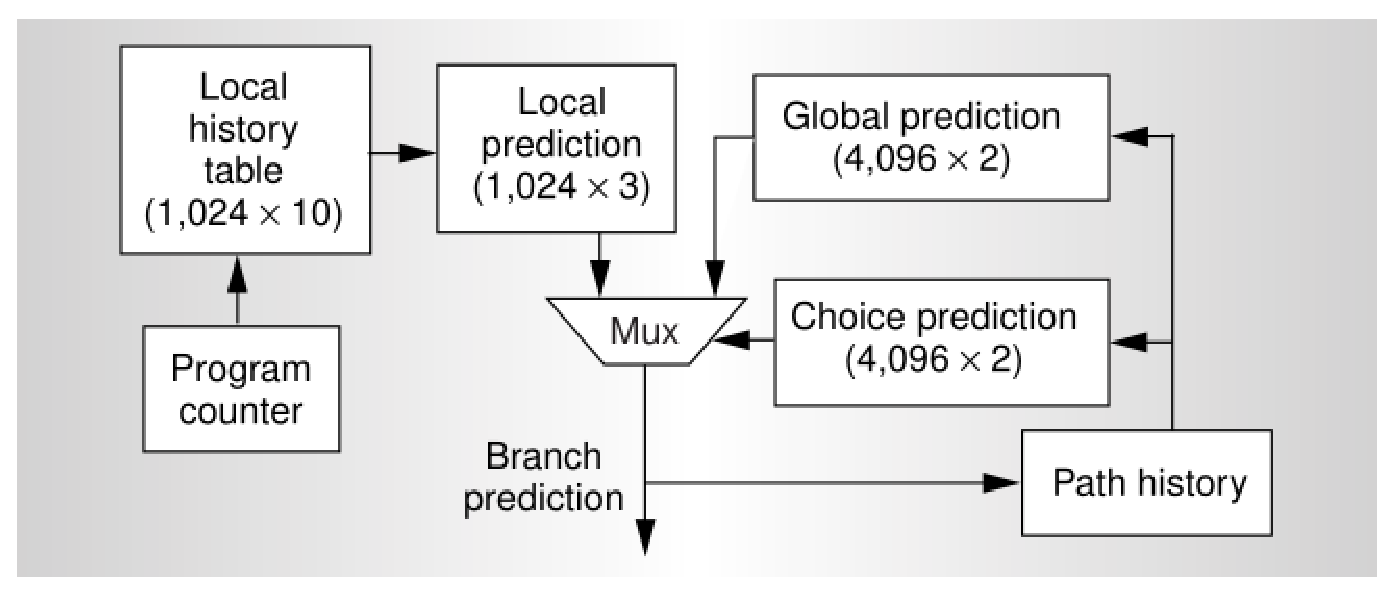
\includegraphics[width=4.5in]{block_diagram.eps}
\end{center}

%\caption*{\small 3-bit Synchronous Up/Down Counter~\cite{counter}.}
\caption*{\textit{Tournament predictor block diagram\cite{kessler}}}
\label{block-diagram}
\end{figure}

\chapter{Testing}
This is a list of branch tests

Reorganize this so it's not just a sea of text and reword for the report\cite{kessler}

\begin{enumerate}[I]
  \item{Testing Initialization}
   %1. Set saturation counters to the following values and get results of tests
      %a. Global  Local  Choice  FP      INT     MM      Notes
          %0       0       0     4.816   12.407  9.795   Strongly not taken/Strongly Local
          %1       3       1     4.724   12.234  9.798   Weakly not taken/Weakly Local
        %* 2       4       0     4.433   11.253  9.094   Weakly taken/Strongly Local
          %2       4       1     4.430   11.265  9.093   Weakly taken/Weakly Local
          %2       4       2     4.431   11.279  9.093   Weakly taken/Weakly Global
          %2       4       3     4.434   11.269  9.098   Weakly taken/Strongly Global
          %3       7       3     4.547   12.512  9.141   Strongly taken/Strongly Global
          %* represents chosen initialization
          %Note: this was done before everything was completely tested, so it could probably be
          %rerun to verify that it really is the best optimization.
  \item{Test functionality of each predictor}
    %1. While working on the patterns for each test I found that I could sufficiently test all
       %branch predictors with one longer test.  This test that shows all the expected results
       %can be found in the spreadsheet. Below are my orignal testing thoughts that turned in
       %to what I actually did that is in the spreadsheet.
       %Note: I still need to update the state transition diagrams because there was a slight
       %change that I had found after speaking with Faust that I hadn't updated and sent out.
    %2. Local Prediction Table
       %a. 3-bit saturation counter works accordingly
          %i. Trains to the correct pattern of prediction (initialized to weakly taken)
             %1. Test that it stays taken by giving it multiple branches that will test each
                %direction of the counter of the taken side. (Assuming that if it worked on one
                %side it will work on the other also.)
                %a. Pattern for actual outcome of branch
                   %i. TTTTNNNTTTT
                      %Note: first branches tests that it goes to strongly taken.
                      %Note: next three test to see that it goes back to weakly taken.
                   %ii. Expected results are found in the spreadsheet 
            %2. Test that it switches from taken to not-taken by giving it multiple branches that
               %are first taken then not taken and back again to check both directions.
               %a. Pattern for actual outcome of branch
                  %i. NNTTTNNNN
               %b. Aliasing
                  %i. Multiple branches go to the same sat. counter.  This is not really ideal
                     %but is necessary due to constraints.
    %3. Global Prediction Table
       %a. 2-bit saturation counter works accordingly
          %i. Trains to the correct pattern of prediction (initialized to weakly not taken)
             %1. Test that it stays not taken by giving it multiple branches that are all actually
                %not taken.
                %a. Pattern needed for preloading the path history to ensure use of the same
                   %counter
                   %i. Just go with 0 everytime it goes through
                %b. Pattern for actual branch outcome
                   %i. NTNNTNNTNN
             %2. Test that it switches from not-taken to taken by giving it multiple branches that
                %are first not-taken and then taken.
                %a. Pattern for preloading path history is the same as above
                %b. Pattern for actual branch outcome
                   %i. NTTTNNTNTT
       %b. Aliasing
          %i. Multiple branches go to the same sat. counter.
    %4. Choice Prediction Table
       %a. 2-bit saturation counter works accordingly
          %i. Trains to the correct pattern of prediction (initialized to weakly local)
             %1. First the path history must be preloaded to ensure it goes to the same sat
                %counter each time.
             %2. Test that it stays local by giving it multiple branches that local would be
                %correct in its prediction and then switch to global.
                %a. Pattern for actual branch outcome
                   %i. NNNNNNTTTTTT
             %3. Test that it switches from local to global by giving it multiple branches that
                %would cause it to switch back and forth between predictors
                %a. Pattern for actual branch outcome
                   %i. NNNNTT
                      %Note: the first 4 are not taken so that it will put both 
                            %L and G predictors to strongly not taken, but because it only
                            %takes two incorrect branches for the global predictor to switch
                            %to taken it is possible to get the global predictor to predict
                            %correctly before the local predictor

\end{enumerate}

\chapter{Source Code}
\section{main.cc}
\lstinputlisting{../src/main.cc}
\pagebreak

\section{predictor.cc}
\lstinputlisting{../src/predictor.cc}
\pagebreak

\bibliographystyle{plain}
\bibliography{kessler}
\end{document}
